% ----------------------------------
% Cap Diseño
% ----------------------------------
%	Incluye
%		Diseño de interfaces y prototipos
%	    
%
\documentclass[a4paper,oneside,11pt]{book}

\usepackage[spanish,activeacute]{babel}
\usepackage[utf8]{inputenc}
%\usepackage[T1]{fontenc}
\usepackage{tabulary}
\usepackage{graphicx}

\usepackage{float}

\setcounter{secnumdepth}{3}

\oddsidemargin=0.2cm
\headsep=1cm
\textheight=21cm
\textwidth=16cm

% Personalizamos la separación entre párrafos...
\parskip=6pt

% Personalizamos el identado en la primera línea del nuevo párrafo...
\parindent=10pt

\begin{document}
% cuerpo del documento
\title{Metodolog'ia de Desarrollo Software}
\author{Pablo Eduardo Ojeda Vasco}
\date{\today}



	\maketitle
%
% Capítulo Diseño de interfaz de usuario
%
\chapter{Diseño} % (fold)
	\label{sec:diseno}

	\section{Diseño de la interfaz de usuario} % (fold)
	\label{sec:interfaz_usuario}
	
	% section diseño_de_la_interfaz_de_usuario (end)
	\subsection{Introducción} % (fold)
		\label{sub:iu_introduccion}
	
	El diseño de la \textbf{interfaz de usuario} crea un medio eficaz de comunicación entre los seres humanos y el ordenador. Siguiendo un conjunto de principios de diseño de la interfaz, el diseño identifica los objetos y acciones de ésta y luego crea una plantilla de pantalla que constituye la base del prototipo de la interfaz de usuario.
	
	La interfaz de usuario de una \textit{webapp} es la \textbf{primera impresión} que se recibe. Sin importar el valor de su contenido, ni la sofisticación de sus capacidades y servicios de procesamiento, así como el beneficio general de la \textit{webapp} en sí, una interfaz mal diseñada decepcionará al usuario potencial y en realidad hará que éste vaya a cualquier otro sitio. Esto ocurre porque las \textbf{interfaces eficaces son atractivas visualmente y perdonan los errores}, lo que da a sus usuarios la sensación de tener el control. Los usuarios perciben rápidamente la totalidad de sus opciones, captan cómo lograr sus metas y cómo hacer su trabajo.
	
	% subsection introduccion (end)
	
	\subsection{Fundamentos para el diseño de las interfaces} % (fold)
	\label{sub:iu_fundamentos}
	
	Cuando se toman decisiones en el diseño de las interfaces de usuario, deben tenerse en cuenta las capacidades físicas y mentales de las personas que utilizarán el software, debido a una serie de \textit{factores humanos} que deben considerarse, cómo son:
	\begin{itemize}
		\item Las personas tienen una memoria limitada a corto plazo.
		\item Todos cometemos errores, especialmente cuando tenemos que manejar demasiada información o estamos estresados.
		\item Tenemos diferentes preferencias de interacción.
		\item Poseemos distintas capacidades físicas (vista, oído, movilidad, etcétera).
	\end{itemize}
	\paragraph{Reglas de oro} % (fold)
	\label{par:reglas_de_oro}
	
	% paragraph reglas_de_oro (end)
	Para el desarrollo de las interfaces vamos a seguir las tres reglas de oro:
	\begin{enumerate}
		\item Dejar el control al usuario.
		\item Reducir la carga de memoria del usuario.
		\item Hacer que la interfaz sea consistente.
	\end{enumerate}
	
	Además, nos vamos a apoyar en una serie de principios de diseño de interfaces de usuario basados en los factores humanos descritos anteriormente. 
	\begin{itemize}
		\item \textit{Familiaridad del usuario}. La interfaz debe utilizar términos y conceptos obtenidos de la experiencia que más utilizan el sistema.
		\item \textit{Uniformidad}. Siempre que sea posible, la interfaz debe ser uniforme en el sentido de que las operaciones comparables se activen de la misma forma.
		\item \textit{Mínima sorpresa}. El comportamiento del sistema no debe provocar sorpresa a los usuarios.
		\item \textit{Recuperabilidad}. La interfaz debe incluir mecanismos para permitir al usuario recuperarse de los errores.
		\item \textit{Diversidad de usuarios}. La interfaz debe proporcionar características de interacción apropiadas para los diferentes tipos de usuario.
	\end{itemize}
	
	Por último y no menos importante, al tratarse de una interfaz para una \textit{webapp}, esta debe responder siempre a tres preguntas principales del usuario final.
	\begin{enumerate}
		\item \textit{¿Dónde estoy?} La interfaz debe dar una indicación de la \textit{webapp} a la que se ha accedido \footnote{Todos hemos marcado una página web y cuando regresamos tiempo después no tenemos una indicación del sitio web o del contexto para la página (ni la manera de pasar a otro sitio.)}y debe informar al usuario de su localización en la jerarquía del contenido.
		\item \textit{¿Qué puedo hacer ahora?} La interfaz siempre debe ayudar al usuario a entender sus opciones actuales: qué funciones están disponibles, qué vínculos están vivos, qué contenido es relevante, etcétera.
		\item \textit{¿Dónde he estado, hacia dónde voy?} La interfaz debe facilitar la navegación. Para ello, debe indicar al usuario dónde ha estado y las trayectorias que pueden tomarse para moverse a cualquier punto de la \textit{webapp}.
	\end{enumerate}
	
	% subsection fundamentos_para_el_diseño_de_las_interfaces (end)
	
	
	\subsection{Diseño de las interfaces} % (fold)
	\label{sec:iu_diseno}
	
	Una vez realizado el análisis del usuario en capítulos anteriores, se ha desarrollado una comprensión de las tareas que éste realiza, su entorno de trabajo, los otros sistemas que utiliza, etcétera. Lo que ahora nos incumbe es el diseño de las interfaces de usuario y realizar los prototipos de la \textit{webapp}. El diseño y desarrollo de la interfaz de usuario es un proceso iterativo. Aunque los usuarios pueden hablar de las facilidades que necesitan de una interfaz, es muy difícil para ellos ser específicos hasta que ven algo tangible. Por lo tanto, se deben desarrollar \textbf{prototipos del sistema}.
	
	Podemos encontrar lo referente a los distintos interfaces de usuario y prototipos de la aplicación dividido en cinco secciones principalmente.
	\begin{itemize}
	\item \textbf{Interfaz Pública.} Interfaz a la que puede acceder cualquier usuario que acceda al sistema. Ésta tiene dos funciones. Por un lado mostrar a los visitantes la funcionalidad del sistema ofreciendo diversas opciones, entre las que cabe destacar la posibilidad de realizar un tour por la aplicación. Por otro lado, es la que ofrece todo lo referente al registro y al acceso.
	\item \textbf{Interfaz Médicos.} Para acceder a ella es necesario haberse registrado como médico. Ofrece a los especialistas todo lo necesario para gestionar sus horarios, pacientes, gestión del centro y otras características que se verán a continuación.
	\item \textbf{Interfaz Pacientes.} Un usuario debe estar registrado como paciente para poder acceder a ella. Ofrece todo lo necesario para gestionar sus citas, médicos, historia clínica y otras características que se verán a continuación.
	\item \textbf{Interfaz Fichas médicas.} Aquí reside gran parte de la información, y su contenido es el de mayor importancia. Es común a médicos y pacientes, aunque con una pequeña diferencia que se añade en la vista del médico.
	\item \textbf{Interfaz Administrador.} Accesible únicamente por el administrador del sistema. Permite, entre otras cosas, dar de alta o de baja a los médicos.
	\end{itemize}
	
	%
	% Subsection Interfaz pública
	%
	\subsubsection{Interfaz pública} % (fold)
		\label{sub:interfaz_publica}
		
		La interfaz pública es aquella a la que pueden acceder tanto usuarios registrados en el sistema cómo usuarios genéricos que todavía no hayan ingresado. En ella encontramos, principalmente, la pantalla de inicio, varios interfaces en los que se muestran las características de la aplicación y por último lo referente al registro y el acceso.
		
		\subparagraph{Pantalla de inicio} % (fold)
		\label{par:pantalla_de_inicio}
		
		La pantalla de inicio (Figura \ref{fig:pantalla_de_inicio}) es con lo que se encontrará el usuario al teclear el nombre del domino de la aplicación en cualquier navegador. En ella destacan un gran \textit{slideshow} \footnote{Pase de diapositivas} con información varia, la posibilidad de buscar un médico para saber si forma parte del sistema, y las opciones de registrarse como paciente o como médico. Además, ofrece una serie de características que se muestran tanto en el menú superior derecho cómo en la parte inferior de la pantalla. Éstas son, el Tour, el Contacto con el administrador, un apartado de preguntas frecuentes, el inicio de sesión, los términos legales y las condiciones de uso. Se han distribuido así debido a que en lo que se quiere hacer mayor énfasis en es captar usuarios, por ello, los cuadros de registro son tan grandes, y ese es el motivo del gran \textit{slideshow} que aparece abarcando la mayor parte de la pantalla. Además, el hecho de que cualquier persona pueda ver si un médico ya forma parte del sistema es muy interesante para captar pacientes, y cuanto mayor sea el número de pacientes, mayor será el número de médicos interesados.
	
		
		\begin{figure}[H]
		  \centering
		    \includegraphics[width=15cm]{img/eps/1_Inicio.eps}
		  \caption{Pantalla de Inicio}
		  \label{fig:pantalla_de_inicio}
		\end{figure}
		% paragraph pantalla_de_inicio (end)	
			
		\subparagraph{Tour de la aplicación} % (fold)
		\label{par:tour_de_la_aplicacion}
		
		Podemos ver el Tour de la aplicación (Figura \ref{fig:tour}), en el que se introducirá al usuario en  una serie de funcionalidades llamativas y útiles, tanto para médicos como para pacientes. Aparecen, entre otras, lo referente a la gestión del centro médico (horarios, pacientes, etcétera), la posibilidad de recibir notificaciones vía email de diversos sucesos, tener toda la información en la nube y poder exportar los datos en cualquier momento, que el paciente gestione sus propias citas y algunas otras.
		
			\begin{figure}[H]
			  \centering
			    \includegraphics[width=12cm]{img/eps/4_Tour.eps}
			  \caption{Tour de la aplicación}
			  \label{fig:tour}
			\end{figure}
			
		% paragraph tour_de_la_aplicación (end)		
		
		\subparagraph{Contacto} % (fold)
		\label{par:contacto}
			La página de contacto (Figura \ref{fig:contacto}) muestra al usuario la dirección de \textit{facebook} y de \textit{twiter} para que puedan hacer un seguimiento de las novedades de la aplicación. Además, muestra información varia acerca de la localización y un formulario desde el que enviar un email directamente al administrador. Por último, sigue ofreciendo la posibilidad de registrarse como médico o como paciente.
		% paragraph contacto_con_el_administrador (end)
		
		\subparagraph{Términos legales, Condiciones de uso y Preguntas frecuentes} % (fold)
		\label{par:terminos_legales_y_condiciones_de_uso}
			Son páginas estáticas en las que se muestra información importante e interesante. Las dos primeras hacen referencia a términos legales y a la protección de datos. La tercera se encarga de, mediante una serie de preguntas/respuestas, informar al usuario de las principales dudas que puedan surgir.
		% paragraph términos_legales_y_condiciones_de_uso (end)
		
		
		\begin{figure}[H]
		  \centering
		    \includegraphics[width=12cm]{img/eps/6_Contacto.eps}
		  \caption{Contacta con MédicalTags}
		  \label{fig:contacto}
		\end{figure}
	
		% subsubsection características (end)
			
	
		% Subsubsection Registro y acceso	
		\subparagraph{Registro y acceso} % (fold)
			\label{par:registro_y_acceso}
	
			Las interfaces para el registro serán distintas en función del rol que ocupemos en el sistema. Para registrarnos cómo pacientes (Figura \ref{fig:registro_paciente}), introducimos nuestro nombre, los datos de acceso y una foto para el perfil. En el caso de registrarnos cómo médicos (Figura \ref{fig:registro_medico}), además deberemos rellenar información de la consulta médica y una serie de datos más específicos, como el número de colegiado, la especialidad, el número de cuenta y, en caso de que se desee, un curriculum. En ambas, antes de registrarte, debes notificar que has leído y que aceptas los términos legales y las condiciones de uso.
			
			La pantalla de acceso (Figura \ref{fig:acceso}) es la misma para cualquier usuario (médico, paciente ó administrador). En ella introducimos nuestro nombre de usuario o email, y la contraseña. Tenemos la opción de recordar contraseña, y de que nos envíen un email en caso de habernos olvidado de ella.
			
			La estructura de las páginas de registro y de acceso es algo diferente a las del resto de la aplicación, eliminando elementos que puedan interferir en el objetivo que nos interesa: registrarse o acceder. Hay que destacar que para el acceso, el identificador de usuario viene proporcionado tanto por el nombre de usuario cómo por el correo electrónico insertado en la fase de registro.
					
			\begin{figure}[H]
			  \centering
			    \includegraphics[width=12cm]{img/eps/3_Registro_Paciente.eps}
			  \caption{Registro de pacientes}
			  \label{fig:registro_paciente}
			\end{figure}
			
			\begin{figure}[H]
			  \centering
			    \includegraphics[width=12cm]{img/eps/2_Registro_Medico.eps}
			  \caption{Registro de médicos}
			  \label{fig:registro_medico}
			\end{figure}
			
			\begin{figure}[H]
			  \centering
			    \includegraphics[width=12cm]{img/eps/5_Acceso.eps}
			  \caption{Acceso}
			  \label{fig:acceso}
			\end{figure}
			
		% subsubsection registro_y_acceso (end)
	% Subsection interfaz_pública (end)
	
	% 
	% Subsectión Panel del médico
	%
	\subsubsection{Panel del médico} % (fold)
		\label{sub:panel_medico}
		
		Cuando un usuario médico inicia sesión por primera vez, la aplicación le muestra un mensaje de bienvenida (Figura \ref{fig:tablero_medico_inicial}) en el que se le recuerda que debe enviar su certificación de licencia médica y configurar su horario. Una vez que haya enviado su licencia, y que el administrador haya acreditado su profesión, sus datos se harán visibles a los pacientes. En los siguientes accesos, se mostrará la sección \textit{Tablero} con la subsección \textit{Ver Resumen}.		
	
		El panel del médico está formado por seis secciones principales.
		\begin{itemize}
			\item Tablero. Ofrece un resumen general y una serie de funcionalidades que se utilizarán frecuentemente.
			\item Calendario. Opciones donde configurar la disponibilidad y ver las citas.
			\item Pacientes. Se muestran los distintos pacientes.
			\item Estadísticas. Permiten al médico ver una serie de detalles sobre la consulta médica en forma de gráficas.
			\item Plantillas. El médico puede elaborar distintos tipos de plantillas predefinidas.
			\item Administración. Todo lo relacionado con la administración y gestión de la consulta médica.
		\end{itemize}
		
		\begin{figure}[H]
		  \centering
		    \includegraphics[width=12cm]{img/eps/7_Dashboar_Medico_Inicial.eps}
		  \caption{Primer acceso del Médico}
		  \label{fig:tablero_medico_inicial}
		\end{figure}
	
		Además, desde el menú superior derecho se podrá cerrar la sesión y acceder a la configuración. Desde esta última, se podrán modificar los datos de contacto, de acceso y otras opciones.
		
		 Por último, cabe destacar que en cualquier momento un médico podrá realizar una búsqueda en el \textit{Vademecum} \footnote{Información sobre medicamentos, sus interacciones e indicaciones.} desde la barra habilitada para ello en la parte superior derecha.
		
		\subparagraph{Tablero} % (fold)
		\label{par:medico_tablero}
		
			En el \textit{Tablero} encontramos una serie de acciones frecuentes e interesantes que los médicos van a realizar. Éstas son \textit{Ver Resumen, Próximas citas, Últimas estadísticas y Buscar Pacientes}.
			
			\textit{Ver Resumen} (Figura \ref{fig:tablero_medico_resumen}) es la pantalla que verá un médico siempre que inicie sesión en el sistema (excepto la primera vez). Ofrece información relevante. Podemos observar que a simple vista vemos los próximos pacientes, y unas estadísticas de pacientes por día y de beneficios. Son datos clave para ver la evolución de su trabajo. Anotar que, con respecto a la lista de los próximos pacientes, el médico verá los próximos pacientes del día a partir de la hora actual. Cuando acabe su turno de trabajo, comenzará a ver los del día siguiente.
		
			\begin{figure}[H]
			  \centering
			    \includegraphics[width=12cm]{img/eps/8_Dashboard_Medico_Tablero.eps}
			  \caption{Tablero médico. Resumen.}
			  \label{fig:tablero_medico_resumen}
			\end{figure}
			
			La pantalla \textit{Próximas citas} (Figura \ref{fig:tablero_medico_citas}) ofrece al médico la posibilidad de ver las próximas X citas que desee.	
			
			\textit{Últimas estadísticas} (Figura \ref{fig:tablero_medico_estadisticas}) muestra una serie de datos del mes actual. Son los pacientes por día que ha tenido la consulta, el porcentaje de los tipos de diagnósticos, los beneficios y el número de pacientes (totales, repetidores, media de repeticiones, etcétera.).
		
			En la subsección \textit{Buscar pacientes} (Figura \ref{fig:tablero_medico_pacientes}), se podrán realizar búsquedas de pacientes en función del \textit{Nombre, DNI, diagnóstico, tratamiento y patología}. El resultado de la búsqueda será una lista ordenada. En ella, se podrá acceder a la ficha médica del paciente, bien haciendo doble click en el nombre, bien desde el botón habilitado para ello. Los cuadrados que se ven en la interfaz son \textit{radio buttons}, es decir, sólo permiten tener seleccionado uno a la vez. También se puede hacer click en el botón \textit{enviar email}.
			
			Todas estas opciones que aparecen en el \textit{Tablero}, están implementadas en las diversas secciones de la interfaz, pero para dar mayor sensación de control y accesibilidad al usuario, se han situado aquí.
			
			\fbox{\parbox{15cm}{En futuras versiones de la aplicación, lo ideal sería que fuera el propio usuario el que pudiera añadir o eliminar funciones del \textit{Tablero}, para adaptarlo lo mejor posible a sus necesidades.}}
			
			\begin{figure}[H]
			  \centering
			    \includegraphics[width=12cm]{img/eps/9_Dashboard_Medico_Tablero_Citas.eps}
			  \caption{Tablero médico. Próximas citas.}
			  \label{fig:tablero_medico_citas}
			\end{figure}
			
			\begin{figure}[H]
			  \centering
			    \includegraphics[width=12cm]{img/eps/10_Dashboard_Medico_Tablero_Estadisticas.eps}
			  \caption{Tablero médico. Últimas estadísticas.}
			  \label{fig:tablero_medico_estadisticas}
			\end{figure}
			
			\begin{figure}[H]
			  \centering
			    \includegraphics[width=12cm]{img/eps/11_Dashboard_Medico_Tablero_Paciente.eps}
			  \caption{Tablero médico. Buscar Pacientes.}
			  \label{fig:tablero_medico_pacientes}
			\end{figure}
		
		
		% subsubsection Tablero (end)
		
		\subparagraph{Calendario} % (fold)
		\label{par:medico_calendario}
		
			En esta sección aparece todo lo relacionado con los horarios del médico, sus citas y una serie de opciones para realizar la configuración  más conveniente.
			
			Por defecto, lo primero con lo que nos encontramos es con la \textit{Vista semanal} (Figura \ref{fig:calendario_vista_semanal}). Ofrece una tabla cuyas columnas son los días de la semana y sus filas secciones equiespaciadas de franjas horarias. Las celdas de la tabla pueden estar vacías en el caso de que no haya ninguna cita concertada con ningún paciente, o pueden tener contenido, en cuyo caso aparecerá el nombre del paciente y el color de fondo será diferente para que resalte sobre las celdas vacías. Podemos ver los datos del paciente que nos interese, bien haciendo doble click sobre la celda en la que se encuentre, o bien seleccionándola y utilizando el botón habilitado para ello (\textit{Ver historia Clínica}). 
			
			Otra posibilidad es la de \textit{Anular Cita}. Con ella se abrirá una ventana en la redactar el texto que le llegará al paciente con la notificación correspondiente. Otra posibilidad es mandar un mensaje por defecto que se podrá establecer en el panel de configuración. Con cualquiera de las dos opciones se pedirá confirmación.			
			
				\fbox{\parbox{15cm}{La vista mensual y la vista diaria, de momento, están previstas para futuras versiones de la aplicación.}}
			
			\begin{figure}[H]
			  \centering
			    \includegraphics[width=12cm]{img/eps/13_Calendario_Medico.eps}
			  \caption{Calendario Médico. Vista Semanal.}
			  \label{fig:calendario_vista_semanal}
			\end{figure}
			
			La \textit{Configuración del horario} (Figura \ref{fig:calendario_configuracion}) es algo que todo médico debe hacer desde que comience a utilizar la aplicación. Otra manera de acceder es desde el menú de \textit{Configuración}, en la parte superior derecha de la pantalla. 
			Existen dos tipos de configuraciones, la estándar y la avanzada. En la primera, el médico establecerá una serie de datos básicos para establecer su horario, como son, los intervalos de duración de sus consultas, los días de trabajo, el tipo de turno (si es de mañana, de tarde o ambos), y las franjas horarias de disponibilidad que oferta a sus pacientes. También hay que introducir el precio medio que establece por realizar su función como especialista sanitario.
			
				\fbox{\parbox{15cm}{La configuración avanzada, de momento, esta prevista para futuras versiones. En ella, un médico podrá establecer días concretos con sus franjas horarias, así podrá, por ejemplo, trabajar lunes y martes por la mañana, y miércoles y jueves por la tarde.}}
				
				Si por cualquier motivo, un día concreto el médico no puede pasar consulta, para no tener que estar anulando las citas una a una, puede hacer uso de la funcionalidad \textit{Anular día} (Figura \ref{fig:calendario_anular_dia}). Esta opción muestra una pantalla en la que elegiremos el día que se desea anular, y un cuadro de texto en el que escribir la notificación que recibirá el paciente. También se puede hacer uso de las que se han establecido por defecto.
				
					\fbox{\parbox{15cm}{Aunque de momento está pensado para futuras versiones, se quiere ofrecer la opción de anular rangos de días. Será muy útil, por ejemplo, si un médico se va de vacaciones.}}
			
			\begin{figure}[H]
			  \centering
			    \includegraphics[width=12cm]{img/eps/15_Calendario_Medico_Configuracion.eps}
			  \caption{Calendario Médico. Configuración.}
			  \label{fig:calendario_configuracion}
			\end{figure}
			
			\begin{figure}[H]
			  \centering
			    \includegraphics[width=12cm]{img/eps/14_Calendario_Medico_Anular.eps}
			  \caption{Calendario Médico. Anular un día concreto.}
			  \label{fig:calendario_anular_dia}
			\end{figure}
			
			La última posibilidad que ofrece el calendario es la de \textit{Configurar las Notificaciones} (Figura \ref{fig:calendario_notificaciones}). Para ello se muestra un menú con \textit{Checkboxs} en donde se seleccionarán las opciones que se desee. Luego habrá que \textit{Guardar}. 
			
			Se ofrecen, en principio, las siguientes posibilidades:
			\begin{itemize}
				\item Cuando un paciente se asigne una cita.
				\item Un día antes de tener una cita.
				\item Cuando un paciente anula una cita.
				\item Cuando un paciente abone una cita.
				\item Cuando se modifique el horario.
				\item Cuando anule una cita.
				\item Cuando un paciente añada una prueba pendiente.
			\end{itemize}
			
				\fbox{\parbox{15cm}{En futuras versiones de la aplicación, estas opciones podrán ampliarse en función de las necesidades que se vayan observando.}}
			
			\begin{figure}[H]
			  \centering
			    \includegraphics[width=12cm]{img/eps/16_Calendario_Medico_Notificaciones.eps}
			  \caption{Calendario Médico. Notificaciones.}
			  \label{fig:calendario_notificaciones}
			\end{figure}
			
			
		% subsubsection calendario (end)
		
		\smallskip
		\subparagraph{Pacientes} % (fold)
		\label{par:medico_pacientes}
		
		En esta sección, un médico podrá encontrar todo lo relacionado con la búsqueda y vista rápida de pacientes.
		
		Tenemos cuatro opciones principales.
		
		\begin{itemize}
			\item \textit{Ver pacientes}. Aparece una lista, en la que se muestran primero los apellidos y luego el nombre, ordenada por orden alfabético, con todos los pacientes que ha tenido un médico. Además, podrá ir directamente a la letra que más le convenga (Figura \ref{fig:pacientes_medico}).
			\item \textit{Buscar pacientes}. Es exactamente la misma opción que vimos en el \textit{Tablero}, en la Figura \ref{fig:tablero_medico_pacientes}. Se podrán realizar búsquedas de pacientes en función del \textit{Nombre, DNI, diagnóstico, tratamiento y patología}. El resultado de la búsqueda será una lista ordenada. En ella, se podrá acceder a la ficha médica del paciente, bien haciendo doble click en el nombre, bien desde el botón habilitado para ello.
			\item \textit{Ver próximos pacientes}. Esta opción también la vimos en el \textit{Tablero} (Figura \ref{fig:tablero_medico_citas}). Ofrece la posibilidad de ver las próximas X citas.
			\item \textit{Ver últimos pacientes}. Es la opción contraria a la de \textit{Ver próximos pacientes}. Ofrece una lista con los últimos X pacientes que ha visitado un médico. 
		\end{itemize}
			
		\begin{figure}[H]
		  \centering
		    \includegraphics[width=12cm]{img/eps/17_Pacientes_Medico.eps}
		  \caption{Pacientes. Ver todos los pacientes.}
		  \label{fig:pacientes_medico}
		\end{figure}
		
		% subsubsection pacientes (end)
		
		\medskip
		\subparagraph{Estadísticas} % (fold)
		\label{par:medico_estadisticas}
		
		La sección \textit{Estadísticas} muestra al médico una serie de gráficas con información sobre los pacientes, los diagnósticos y los beneficios. La primera pantalla con la que nos encontramos es la de \textit{Ver últimas estadísticas} (Figura \ref{fig:estadisticas_medico}), que ofrece información detalla del último mes. Es lo mismo que encontramos en el \textit{Tablero}. Muestra una serie de datos del mes actual. Son los pacientes por día que ha tenido la consulta, el porcentaje de los tipos de diagnósticos, los beneficios y el número de pacientes (totales, repetidores, media de repeticiones, etcétera.). Además, se ofrece la posibilidad de \textit{Imprimir}.
		
		Las opciones de \textit{Estadísticas mensuales} y \textit{Estadísticas anuales}, son similares. La diferencia está en que aparecen los datos agrupados, en vez de por días, por meses y por años respectivamente.
		
		\fbox{\parbox{15cm}{En futuras versiones de la aplicación, se pretenden añadir otro tipo de estadísticas que puedan ser interesantes.}}
		
		\fbox{\parbox{15cm}{En futuras versiones de la aplicación, se pretenden añadir estadísticas concretas sobre pacientes, sobre diagnósticos y sobre beneficios.}}
		
		\fbox{\parbox{15cm}{Se pretende añadir la opción de \textit{Exportar estadísticas}, aunque por el momento esto queda para futuras versiones.}}
		
		\begin{figure}[H]
		  \centering
		    \includegraphics[width=12cm]{img/eps/19_Estadisticas_Medicos.eps}
		  \caption{Pacientes. Ver últimas estadísticas.}
		  \label{fig:estadisticas_medico}
		\end{figure}
		
		% subsubsection estadísticas (end)
		
		\bigskip
		\medskip
		\subparagraph{Plantillas} % (fold)
		\label{par:medico_plantillas}
		
		En esta sección se pretende ofertar a los especialistas la posibilidad de elaborar una serie de plantilla predefinidas. Esta opción es realmente útil debido a que favorece notablemente en el ahorro de tiempo. Por ejemplo, si un médico suele dar un tratamiento con frecuencia, un diagnóstico o cualquier otro documento, para evitar tener que estar redactándolo con cada paciente que lo necesite, con la consecuente pérdida de tiempo que ello supone, puede seleccionar el documento de una plantilla y modificar algunos campos como el nombre del paciente, la dosis de la medicación, etcétera.
		
		Las opciones que se ofrecen, todas ellas muy similares, son las de \textit{Elaborar Plantilla (Figura \ref{fig:plantillas_medico}), Modificar Plantilla o Eliminar Plantilla}. En todas ellas aparecerán seis opciones, puesto que vamos a establecer seis tipos de documentos. Estas son:
		
		\begin{itemize}
			\item Plantilla de Diagnóstico.
			\item Plantilla de Tratamiento.
			\item Plantilla de Informe.
			\item Plantilla de Receta.
			\item Plantilla para consulta.
			\item Otras.
		\end{itemize}
		
		\begin{figure}[H]
		  \centering
		    \includegraphics[width=12cm]{img/eps/18_Plantillas_Medico.eps}
		  \caption{Plantillas. Elaborar Plantillas.}
		  \label{fig:plantillas_medico}
		\end{figure}
		
		% subsubsection plantillas (end)
		
		\subparagraph{Administración} % (fold)
		\label{par:medico_administracion}
		
			Un médico podrá tener una serie de datos referente a la administración y gestión de su consulta médica. La pantalla inicial que aparece al acceder a esta sección es la de \textit{Historial} (Figura \ref{fig:administracion_historial}
			
			Las distintas opciones con las que nos encontramos son:
			
			\begin{itemize}
				\item \textit{Historial}. En ella se ofrece una lista que abarca todo lo que ha ocurrido en la consulta: ingresos, gastos, diagnósticos u otros documentos generados, citas concertadas, citas anuladas, notificaciones enviadas, etcétera. Se pueden ver los detalles de cada una de las entradas de la lista, imprimirla o exportarla.
				
					\fbox{\parbox{12cm}{De momento, la opción \textit{Exportar} está pensada para futuras versiones.}}
				
					\begin{figure}[H]
				  		\centering
				    	\includegraphics[width=12cm]{img/eps/22_1_Administracion_Historial_Medico.eps}
				  		\caption{Administración. Historial.}
				  		\label{fig:administracion_historial}
					\end{figure}
				
				\item \textit{Añadir gasto} (Figura \ref{fig:administracion_gasto}). Una consulta médica también tiene gastos de diversos tipos (mantenimiento, agua, luz, gestoría, ayuntamientos, etcétera). Lo ideal para llevar una buena gestión de la contabilidad es anotar todos los gastos. El médico debe seleccionar la fecha en la que se realizó el gasto, añadir el motivo, seleccionar la cantidad y documentar un comentario en caso de que sea necesario. Si se dispone de factura digital, podrá adjuntarla directamente. En caso de no disponer de ella, podrá escanearla y adjuntarla. Anotar que los motivos están predefinidos por el especialista, y que se pueden añadir o eliminar motivos en cualquier momento desde el panel de \textit{Configuración} situado en la parte superior derecha.
				
				\begin{figure}[H]
				  \centering
				    \includegraphics[width=12cm]{img/eps/20_Administracion_Medico.eps}
				  \caption{Administración. Añadir Gasto.}
				  \label{fig:administracion_gasto}
				\end{figure}
				
				\item \textit{Añadir ingreso} (Figura \ref{fig:administracion_ingreso}). En el caso de que un paciente pague por adelantado, automáticamente se generará una factura y se anotará en los ingresos y en las facturas emitidas. Sin embargo, si un paciente paga al finalizar la consulta, será el médico el que se encargue de anotar el ingreso. Para ello debe seleccionar la fecha, añadir el motivo, establecer la cantidad, asociarlo a un paciente y añadir un comentario en caso de ser necesario. Finalmente, generará una factura que se le enviará al paciente y que se guardará en el historial junto con el ingreso realizado.
				\item \textit{Balance global} (Figura \ref{fig:administracion_balance}). Muestra una serie de datos sobre ingresos totales, netos, brutos y gastos.
				\item \textit{Facturas emitidas}. Muestra una lista de las últimas facturas emitidas. Permitirá búsquedas por rango de fechas.
				\item \textit{Facturas recibidas}. Muestra una lista de las últimas facturas recibidas. Permitirá búsquedas por rango de fechas.
				\item \textit{Buscar facturas}. Permite utilizar diversos filtros de búsqueda para encontrar la factura deseada, como son fecha, paciente, motivo, cantidad, etcétera.
				\item \textit{Ver votos}. Una vez finalizada la consulta, un paciente podrá valorar la actuación del médico. Para ver los últimos votos recibidos, se utilizará esta opción.				
			\end{itemize}
			
		\fbox{\parbox{15cm}{La opción \textit{Ver votos} se implementará en futuras versiones.}}
		
		\begin{figure}[H]
		  \centering
		    \includegraphics[width=12cm]{img/eps/21_Administracion_Medico2.eps}
		  \caption{Administración. Balance Global.}
		  \label{fig:administracion_balance}
		\end{figure}
		
		\begin{figure}[H]
		  \centering
		    \includegraphics[width=12cm]{img/eps/22_Administracion_Medico1.eps}
		  \caption{Administración. Añadir Ingreso.}
		  \label{fig:administracion_ingreso}
		\end{figure}
				
		% subsubsection administración (end)
		
		\subparagraph{Configuración} % (fold)
		\label{par:medico_configuracion}
		
		La última sección que encontramos en los interfaces del médico es la de \textit{Configuración}. Para acceder a ella debemos hacer click en la parte superior derecha de la pantalla. La subsección de \textit{Datos} es lo primero que aparece cuando accedemos a esta sección. Las distintas posibilidades que podemos encontrar son las siguientes:
		
		\begin{itemize}
			\item \textit{Datos} (Figura \ref{fig:configuracion_datos}). Hace referencia a los datos personales del médico y de su consulta médica. La información que se muestra es su nombre, su email, su número de colegiado, datos de contacto y de localización y un número de cuenta. También se puede ver la foto de su perfil, añadirla en caso de no tener ninguna, o modificarla en caso de querer cambiar la actual. Cabe destacar que, además, se permite al médico ver su curriculum, adjuntarlo si no lo ha hecho todavía, crearlo y modificarlo. Todos los datos podrán ser cambiados en cualquier momento que se desee.
			
			\fbox{\parbox{15cm}{La opción \textit{Crear Curriculum} se implementará en futuras versiones. Por su parte, la opción de \textit{Añadir curriculum}, de momento, sólo permitirá añadir un documento .pdf, y la de \textit{Modificar Curriculum} simplemente cambiará un .pdf por otro.}}
			
			\begin{figure}[H]
			  \centering
			    \includegraphics[width=12cm]{img/eps/23_Configuracion_Medico.eps}
			  \caption{Configuración Médico. Datos.}
			  \label{fig:configuracion_datos}
			\end{figure}
			
			\item \textit{Cuenta} (Figura \ref{fig:configuracion_cuenta}). Como toda aplicación Web, los datos de la cuenta de cualquier usuario deben poder modificarse. En ésta no iba a ser diferente. Podemos cambiar el nombre de usuario, la contraseña, el idioma o darnos de baja en el servicio.
			
			\begin{figure}[H]
			  \centering
			    \includegraphics[width=12cm]{img/eps/24_Configuracion_Medico2.eps}
			  \caption{Configuración Médico. Cuenta.}
			  \label{fig:configuracion_cuenta}
			\end{figure}
			
			\item \textit{Horario}. La configuración del horario es la misma que veíamos desde la sección \textit{Calendario}. Más concretamente en la opción \textit{Configuración del horario} (Figura \ref{fig:calendario_configuracion}). En él se establecían una serie de datos clave para elaborar la disponibilidad del médico e informar de ella a los posibles pacientes. Entre otras, los días laborables, los rangos horarios de trabajo, la duración de las consultas, etcétera.
			
			\item \textit{Enviar certificado}. Es algo que todo médico debe hacer si quiere que sus posibles pacientes (otros usuarios del sistema) puedan ver su información y la de su horario de disponibilidad. Lo único que debe hacer es mandar la certificación de licencia médica al administrador, y en cuanto éste la verifique, podrá comenzar comenzar a sacar partido de las diversas funcionalidades que se le ofrecen.
			
			\item \textit{Notificaciones}. En esta opción permitimos al médico dos cosas. En primer lugar configurar las notificaciones, tal y cómo se vio en la sección \textit{Calendario} (Figura \ref{fig:calendario_notificaciones}). En segundo lugar establecer los mensajes por defecto que recibirán sus pacientes en caso de que se anule una consulta por parte del médico.
			
			\item \textit{Motivos}. Permite al médico configurar una lista con los posibles motivos que se pueden añadir a la hora de generar una factura o de anotar un gasto.
			
		\end{itemize}
				
		% subsubsection configuración (end)
		
	% subsection Panel del médico (end)
	
	%
	% Subsection Panel del paciente
	%
	\bigskip
	\subsubsection{Panel del paciente} % (fold)
		\label{sub:panel_paciente}
	
		Cuando un usuario paciente inicia sesión por primera vez, la aplicación le muestra un mensaje de bienvenida (Figura \ref{fig:tablero_paciente_inicial}) en el que se le recuerda que lo ideal es que rellene todos los campos posibles de su ficha médica y que adjunte todas las pruebas de las que disponga. Además, le aconseja que realice una primera búsqueda de sus posibles médicos favoritos. En los siguientes accesos, se mostrará la sección \textit{Tablero} con la subsección \textit{Ver Resumen}.		
	
		El panel del médico está formado por cinco secciones principales.
		\begin{itemize}
			\item Tablero. Ofrece un resumen general y una serie de funcionalidades que se utilizarán frecuentemente.
			\item Calendario. Opciones donde ver las citas que tiene previstas.
			\item Médicos. Se realiza la búsqueda de médicos en función de diversos filtros y se asignan las citas.
			\item Ficha médica. Contiene todo lo referente a los datos sanitarios del paciente.
			\item Historial. Una lista que abarca todo lo que ha ocurrido con el paciente: pago de consultas, diagnósticos u otros documentos recibidos, citas concertadas, citas anuladas, notificaciones recibidas, etcétera. 
		\end{itemize}
		
		\begin{figure}[H]
		  \centering
		    \includegraphics[width=12cm]{img/eps/25_Tablero_Paciente.eps}
		  \caption{Primer acceso del Paciente}
		  \label{fig:tablero_paciente_inicial}
		\end{figure}
	
		Además, desde el menú superior derecho se podrá cerrar la sesión y acceder a la configuración. Desde esta última, se podrán modificar los datos de contacto, de acceso y otras opciones.
		
		 Por último, cabe destacar que en cualquier momento un paciente podrá realizar una búsqueda sobre \textit{Terminología médica} desde la barra habilitada para ello en la parte superior derecha.
	
		\subparagraph{Tablero} % (fold)
		\label{par:paciente_tablero}
		En el \textit{Tablero} encontramos una serie de acciones frecuentes e interesantes que los pacientes van a realizar. Éstas son \textit{Ver Resumen, Médicos favoritos, y Añadir datos}.
		
		\textit{Ver Resumen} (Figura \ref{fig:tablero_paciente_resumen}) es la pantalla que verá un paciente siempre que inicie sesión en el sistema (excepto la primera vez). Ofrece información relevante. Podemos observar que a simple vista vemos una lista con el tratamiento actual (la medicación y la dosis diaria que debe tomar), su último diagnóstico (y el médico que lo ha generado), las pruebas que tiene pendientes de realizarse y cuáles son sus próximas citas, indicando la hora y el médico.
	
		\begin{figure}[H]
		  \centering
		    \includegraphics[width=12cm]{img/eps/26_Tablero_Paciente1.eps}
		  \caption{Tablero Paciente. Resumen.}
		  \label{fig:tablero_paciente_resumen}
		\end{figure}
		
		La pantalla \textit{Médicos favoritos} ofrece al paciente la posibilidad de ver sus especialistas preferidos, para ir directamente a su horario de disponibilidad.	
		
		\textit{Añadir datos} lleva al paciente directamente a la parte de la historia clínica y a la pestaña pruebas, para desde ella añadirla en función de su tipo.
		
		\fbox{\parbox{15cm}{En futuras versiones de la aplicación, lo ideal sería que fuera el propio usuario el que pudiera añadir o eliminar funciones del \textit{Tablero}, para adaptarlo lo mejor posible a sus necesidades.}}
		
		% subsubsection tablero (end)
		
		\subparagraph{Calendario} % (fold)
		\label{par:paciente_calendario}
		
		En esta sección aparece todo lo relacionado con las citas previstas del paciente y una serie de opciones para realizar la configuración  más conveniente.
		
		Por defecto, lo primero con lo que nos encontramos es con la \textit{Vista semanal} (Figura \ref{fig:calendario_vista_semanal_paciente}). Ofrece una tabla cuyas columnas son los días de la semana y sus filas secciones equiespaciadas de franjas horarias. Las celdas de la tabla pueden estar vacías en el caso de que no haya ninguna cita concertada con ningún médico, o pueden tener contenido, en cuyo caso aparecerá el nombre del médico y el color de fondo será diferente para que resalte sobre las celdas vacías. Podemos ver los datos del médico que nos interese, bien haciendo doble click sobre la celda en la que se encuentre, o bien seleccionándola y utilizando el botón habilitado para ello (\textit{Ver datos del médico}). 
		
		Otra posibilidad es la de \textit{Anular Cita}. Se pedirá confirmación.			
		
			\fbox{\parbox{15cm}{La vista mensual y la vista diaria, de momento, están previstas para futuras versiones de la aplicación.}}
		
		\begin{figure}[H]
		  \centering
		    \includegraphics[width=12cm]{img/eps/27_Calendario_Paciente.eps}
		  \caption{Calendario Paciente. Vista Semanal.}
		  \label{fig:calendario_vista_semanal_paciente}
		\end{figure}
		
		La \textit{Lista de Próximas Citas} ofrece una vista de los próximos encuentros que tendrá el paciente con el médico. Podrá ver las próximas X citas.		
		
		La última posibilidad que ofrece el calendario es la de \textit{Configurar las Notificaciones}. Es muy similar a lo que veíamos en el calendario del médico. 	
		
		% subsubsection calendario (end)
		
		\subparagraph{Médicos} % (fold)
		\label{par:paciente_medicos}
		
			Esta sección permite al paciente realizar múltiples acciones relacionadas con los médicos. La pantalla inicial será la de \textit{Buscar médico} (Figura \ref{fig:medico_paciente_buscar}). En ella, un paciente podrá utilizar una serie de filtros para encontrar el especialista que más le convenga en función de: \textit{nombre, especialidad, precio, localización, valoración, etcétera.} Una vez que aparezcan los resultados, podrá \textit{ver sus horarios} haciendo doble click sobre el nombre. También puede \textit{ver la información} y \textit{añadirlo a sus médicos favoritos}. 
			
			\fbox{\parbox{15cm}{En futuras iteraciones se propone la posibilidad de realizar \textit{búsquedas avanzadas}.}}
			
			El resto de posibilidades con las que nos encontramos son:
			\begin{itemize}
				\item \textit{Ver favoritos}. Muestra una lista con los médicos favoritos.
				\item \textit{Ver últimos}. Muestra una lista de los últimos médicos con los que ha tenido cita un paciente.
				\item \textit{Ver próximos}. Muestra una lista con los próximos médicos.
				\item \textit{Ver todos}. Muestra una lista con todos los médicos a los que ha asistido.
				\item \textit{Votar médicos}. Permite a un paciente votar a un médico con el que ha tenido alguna cita. Esta opinión pretende aconsejar a futuros pacientes.
			\end{itemize}
		
		\fbox{\parbox{15cm}{\textit{Votar médicos}, de momento, está pensado realizarse en futuras iteraciones.}}
		
			\begin{figure}[H]
			  \centering
			    \includegraphics[width=12cm]{img/eps/28_Medicos_Paciente.eps}
			  \caption{Médicos del Paciente. Buscar médico.}
			  \label{fig:medico_paciente_buscar}
			\end{figure}
		
		% subsubsection médicos (end)
		
		\subparagraph{Historial} % (fold)
		\label{par:paciente_historial}
		
		Una lista que abarca todo lo que ha ocurrido con el paciente: pago de consultas, diagnósticos u otros documentos recibidos, citas concertadas, citas anuladas, notificaciones recibidas, etcétera. 
		
		En principio, aparecerá la lista con toda la información. Sin embargo, se podrán realizar búsquedas en función de lo que se desee.		
		
		% subsection historial (end)
		
		\subparagraph{Configuración} % (fold)
		\label{par:paciente_configuracion}
		
			La última sección que encontramos en los interfaces del paciente es la de \textit{Configuración}. Para acceder a ella debemos hacer click en la parte superior derecha de la pantalla. La subsección de \textit{Datos} es lo primero que aparece cuando accedemos a esta sección. Las distintas posibilidades que podemos encontrar son las siguientes:

			\begin{itemize}
				\item \textit{Datos}. Hace referencia a los datos personales del paciente. 
				\item \textit{Cuenta} (Figura \ref{fig:configuracion_cuenta_paciente}). Como toda aplicación Web, los datos de la cuenta de cualquier usuario deben poder modificarse. En ésta no iba a ser diferente. Podemos cambiar el nombre de usuario, la contraseña, el idioma o darnos de baja en el servicio.

				\begin{figure}[H]
				  \centering
				    \includegraphics[width=12cm]{img/eps/28_1_Cuenta_Pacientes.eps}
				  \caption{Configuración Paciente. Cuenta.}
				  \label{fig:configuracion_cuenta_paciente}
				\end{figure}

				\item \textit{Notificaciones}. En esta opción permitimos al paciente configurar las notificaciones, de forma similar a cómo se vio en la sección \textit{Calendario} del médico (Figura \ref{fig:calendario_notificaciones}). 
			\end{itemize}
		
		% subsubsection configuración (end)
		
	% Subsection Panel del paciente (end)
	
	
	%
	% Subsectión Ficha médica
	%
	\subsubsection{Ficha médica} % (fold)
		\label{sub:ficha_medica}
	
		La ficha médica es uno de los grandes gruesos de la aplicación. Es utilizada tanto por médicos como por pacientes. Por estos motivos se especifican los detalles de su interfaz en este apartado a parte.
		
		Comenzar diciendo que todo paciente tiene una ficha médica en cada uno de los médicos a los que asiste. En esta ocasión, tiene una ficha médica a la que pueden acceder todos sus médicos, evitando así tener información redundante en cada especialista, y además ahorrando al paciente tener que llevar toda su información cada vez que asiste a una nueva consulta.
		
		La vista que tiene el paciente de la ficha médica es la misma que la del médico, salvo por una excepción, el apartado \textit{Observaciones}. Éste apartado no es visible para el primero y no está compartido por distintos especialistas. Es decir, cada médico tendrá sus propias observaciones de cada paciente, visibles únicamente por él mismo. 
		
		Los campos que posee la ficha de un paciente son los que se muestran a continuación. Porteriormente se comentarán con más detalle.
		
		\begin{itemize}
			\item \textit{Información Personal}. Datos personales del paciente.
			\item \textit{Antecedentes}. Enfermedades que ha sufrido, enfermedades genéticas, etcétera.
			\item \textit{Enfermedad actual}. Datos sobre la/s enfermedad/es que sufre actualmente.
			\item \textit{Exploración}. Una serie de datos fisiológicos que se toman durante la consulta.
			\item \textit{Pruebas}. Todo lo relacionado con análisis, radiografías, y una serie de pruebas propias de cada especialidad.
			\item \textit{Diagnósticos}. Los diagnósticos que ha recibido un paciente de los diversos especialistas.
			\item \textit{Tratamientos}. Los tratamientos que ha recibido un paciente de los diversos especialistas.
			\item \textit{Informes}. Los Informes que ha recibido un paciente de los diversos especialistas.
			\item \textit{Historial}. Se almacena todo lo que ocurre en la ficha de un paciente. Cuando se añade una prueba, un diagnóstico, se modifica algún tratamiento, etcétera.
			\item \textit{Observaciones}. Campo que posee cada médico de cada uno de sus pacientes.
		\end{itemize}
		
		En las próximas dos imágenes podemos observar que el paciente tiene su propia sección \textit{Ficha médica} (Figura \ref{fig:hc_paciente}), mientras que los médicos acceden a esta información a partir de cada uno de los pacientes, bien haciendo doble click en su nombre o bien utilizando el botón habilitado para esta función (\textit{Ver historia clínica}) (Figura \ref{fig:hc_medico}).
		
		\begin{figure}[H]
		  \centering
		    \includegraphics[width=12cm]{img/eps/29_1_Historial_Medico.eps}
		  \caption{Historia clínica desde el interfaz del Médico. Observaciones}
		  \label{fig:hc_medico}
		\end{figure}
		
		\begin{figure}[H]
		  \centering
		    \includegraphics[width=12cm]{img/eps/29_Historial_Paciente.eps}
		  \caption{Historia clínica desde el interfaz del Paciente. Información Personal.}
		  \label{fig:hc_paciente}
		\end{figure}
		
		\subparagraph{Antecedentes} % (fold)
		\label{par:antecedentes}
		
			Muestra información relativa a enfermedades anteriores de diversos tipos. Todos los datos se podrán \textit{imprimir y exportar.}
			
			\fbox{\parbox{15cm}{\textit{Imprimir y exportar}, de momento, se realizarán en futuras versiones.}}
			
			Está dividido en tres secciones.
			
			\begin{itemize}
				\item \textit{Antecedentes fisiológicos} (Figura \ref{fig:antecedentes_fisiologicos}). Son una serie de cuestiones sobre las vacunas, la menopausia, las alergias, si practica deportes, alcohol, café, tabaco, etcétera.
				\item \textit{Antecedentes familiares} (Figura \ref{fig:antecedentes_familiares}). Muestra enfermedades genéticas que hayan padecido los padres, los hermanos u algún otro familiar directo. 
				
				\fbox{\parbox{15cm}{Se tiene pensado incluir en futuras versiones una serie de enfermedades típicas para que sea el propio usuario el que las elija, evitando así confusiones.}}
				
				\item \textit{Antecedentes personales} (Figura \ref{fig:antecedentes_personales}). Las enfermedades de distintos tipos que haya padecido el paciente, las operaciones quirúrgicas, los tratamientos, etcétera. 
			\end{itemize}
			
			\subparagraph{Enfermedad actual} % (fold)
			\label{par:enfermedad_actual}
				Es igual que enfermedades anteriores, pero con la información de la/s enfermedad/es actual/actuales.
			% paragraph enfermedad_actual (end)
			
			\begin{figure}[H]
			  \centering
			    \includegraphics[width=12cm]{img/eps/30_Antecedentes_pacientes.eps}
			  \caption{Historia clínica. Antecedentes Fisiológicos.}
			  \label{fig:antecedentes_fisiologicos}
			\end{figure}
			
			\begin{figure}[H]
			  \centering
			    \includegraphics[width=12cm]{img/eps/31_Antecedentes_pacientes1.eps}
			  \caption{Historia clínica. Antecedentes Familiares.}
			  \label{fig:antecedentes_familiares}
			\end{figure}
			
			\begin{figure}[H]
			  \centering
			    \includegraphics[width=12cm]{img/eps/32_Antecedentes_pacientes2.eps}
			  \caption{Historia clínica. Antecedentes Personales.}
			  \label{fig:antecedentes_personales}
			\end{figure}
			
		% paragraph antecedentes (end)
		
		\subparagraph{Exploración} % (fold)
		\label{par:exploracion}
		
			La \textit{Exploración clínica} es realizada por los médicos, aunque hay datos que puede rellenar el propio paciente. 
			
			Es interesante tener conocimiento del peso, la talla, la tensión arterial, el pulso, la temperatura, etcétera. Pueden orientar al médico muchas veces en su diagnóstico.
			
			Así mismo, hay que tener presente si el paciente presenta algún tipo de marca, identificativa de un golpe o una lesión. Las cicatrices también pueden aportar información relevante según qué casos.
			
			Otros datos a tener en cuenta serán las deformidades y la deambulación.
			
			\fbox{\parbox{15cm}{La \textit{Exploración clínica} puede ser diferente según el tipo de especialidad. En principio, los datos que aparecen en la Figura \ref{fig:exploracion} serán los que aparezcan en la aplicación. Sin embargo, en futuras versiones se separarán por especialidad.}}
			
			\fbox{\parbox{15cm}{\textit{Imprimir y exportar}, de momento, se realizarán en futuras versiones.}}
			
			\begin{figure}[H]
			  \centering
			    \includegraphics[width=12cm]{img/eps/33_Exploracion_paciente.eps}
			  \caption{Historia clínica. Exploración.}
			  \label{fig:exploracion}
			\end{figure}
			
		% paragraph exploración (end)
		
		\bigskip
		\bigskip
		\bigskip
		\subparagraph{Pruebas} % (fold)
		\label{par:pruebas}
			
			La cantidad de diferentes tipos posibles de prueba es muy elevada. Cada especialidad dispone de las suyas propias. Por otro lado hay algunas que son genéricas.
			
			De momento, las que se implementarán serán:
	
			\begin{itemize}
				\item \textit{Análisis} (Figura \ref{fig:prueba_analisis}). Lista de los análisis de sangre, orina, heces, etcétera.
				\item \textit{Radiodiagnóstico} (Figura \ref{fig:prueba_radio}). A su vez encontramos cuatro tipos de posibles pruebas radiográficas, como son \textit{radiografías, ecografías \footnote{Imagen que se obtiene mediante una técnica de exploración del interior de un cuerpo mediante ondas electromagnéticas o acústicas, que registra las reflexiones o ecos producidas en su propagación por las discontinuidades internas.}, TAC \footnote{Conjunto de imágenes seriadas de secciones de un órgano o tejido, obtenidas a lo largo de un eje mediante distintas técnicas, y computarizadas.}, y Resonancias magnéticas \footnote{Obtiene imágenes internas de un organismo, especialmente con fines diagnósticos. Utiliza una técnica de absorción de energía por los átomos de una sustancia cuando son sometidos a campos magnéticos de frecuencias específicas.}}
				\item \textit{Histología \footnote{Ciencia que estudia todo lo referente a los tejidos orgánicos: su estructura microscópica, su desarrollo y sus funciones. La histología se identifica a veces con lo que se ha llamado anatomía microscópica, pues su estudio no se detiene en los tejidos, sino que va más allá, observando también las células interiormente y otros corpúsculos, relacionándose con la bioquímica y la citología.}}.
			\end{itemize}
			
			En un futuro se pretende contar, además, con pruebas propias de cada especialidad, como son \textit{Neurológicas, Cardiacas, Renales, Gástricas, Oftalmológicas, etcétera}.
			
			Funcionalmente, todas las pruebas son exactamente iguales. Aparece una lista ordenada por fechas de todas ellas. Existe la posibilidad de:
			
			\begin{itemize}
				\item \textit{Ver la prueba}. Permite al médico o al paciente ver una prueba. Puede utilizarse el botón habilitado para ello o simplemente hacer doble click sobre la que se desee ver.
				\item \textit{Añadir prueba}. Se abrirá una ventana en la que se indique el tipo de prueba que se desea añadir. Cada especialidad podrá elegir entre un tipo de pruebas predefinidas.
				\item \textit{Solicitar prueba}. Indica que existe un estado en el que el médico está pendiente de recibir una prueba que el paciente debe hacerse y que debe añadirse al sistema.
				\item \textit{Imprimir}. 
				\item \textit{Exportar}. 
			\end{itemize}
			
			\fbox{\parbox{15cm}{\textit{Imprimir y exportar}, de momento, se realizarán en futuras versiones.}}
			
			\fbox{\parbox{15cm}{\textit{Solicitar prueba} también tiene pensado realizarse en futuras iteraciones.}}
			
			\begin{figure}[H]
			  \centering
			    \includegraphics[width=12cm]{img/eps/34_Pruebas_Pacientes.eps}
			  \caption{Historia clínica. Pruebas de análisis.}
			  \label{fig:prueba_analisis}
			\end{figure}
			
			\begin{figure}[H]
			  \centering
			    \includegraphics[width=12cm]{img/eps/35_Pruebas_Pacientes2.eps}
			  \caption{Historia clínica. Pruebas radiodiagnósticas.}
			  \label{fig:prueba_radio}
			\end{figure}
				
		% paragraph pruebas (end)
		
		\paragraph{Diagnósticos} % (fold)
		\label{par:diagnosticos}
		
			Se muestra una lista ordenada por fechas de los distintos diagnósticos y del médico que lo diagnosticó. Además, aparece más detallado el último diagnóstico recibido (Figura \ref{fig:diagnostico}). 
			
			Se cuentan con opciones similares a las de las pruebas, como son \textit{ver diagnóstico} \textit{añadir diagnóstico, imprimir y exportar}.
			
			\fbox{\parbox{15cm}{\textit{Imprimir y exportar}, de momento, se realizarán en futuras versiones.}}
			
			\begin{figure}[H]
			  \centering
			    \includegraphics[width=12cm]{img/eps/36_Diagnosticos_Pacientes.eps}
			  \caption{Historia clínica. Diagnósticos.}
			  \label{fig:diagnostico}
			\end{figure}
		% paragraph diagnósticos (end)
		
	% Subsection Ficha médica (end)		
		
	%
	% Subsectión Panel de Administrador
	%
	\subsubsection{Panel del Administrador} % (fold)
		\label{sub:panel_administrador}
	
		El administrador del sistema puede realizar las siguientes funciones:
		
		\begin{itemize}
			\item \textit{Verificar Médico}. Una vez que un médico ha enviado su certificación de licencia médica, será el administrador del sistema el que lo verifique y procede a activarlo para que sea visible por el resto de usuarios.
			\item \textit{Agregar administrador}. Permite añadir otro administrador.
			\item \textit{Eliminar Médico}. Cuando un médico desea darse de baja en el servicio.
			\item \textit{Suspender Médico}. Cuando un médico lleva tiempo sin usar el servicio.
			\item \textit{Reactivar Médico}. Cuando un tiempo que estaba suspendido desea reactivar el servicio.
			\item \textit{Preguntas} (Figura \ref{fig:admin_preguntas}). Aparecen las preguntas enviadas al administrador. Éste puede ver las preguntas completas, eliminar preguntas y contestar a las preguntas.
			\item \textit{Condiciones de Uso}. Permite al administrador modificar fácilmente las condiciones de uso.
			\item \textit{Contacto}. Permite al administrador modificar fácilmente los datos de contacto.
			\item \textit{Términos legales}. Permite al administrador modificar fácilmente los términos legales.
		\end{itemize}
	
		\begin{figure}[H]
		  \centering
		    \includegraphics[width=12cm]{img/eps/99_Administrador.eps}
		  \caption{Panel de Administrador. Preguntas.}
		  \label{fig:admin_preguntas}
		\end{figure}
	
	% subsection Panel de administrador (end)
	% section diseño_de_las_interfaces (end)
\end{document}
% section diseño_de_interfaz_de_usuario (end)
% chapter diseño (end)